\clearpage\begingroup\SourceLeaf{647}
\ArithmeticHead{12}{L}{H. GEPPERT, ÜBER GAUSS’ ARBEITEN ZUR MECHANIK UND POTENTIALTHEORIE.}
\renewcommand{\thefootnote}{\arabic{footnote})}\setcounter{footnote}{15}
\begin{center}\textls[100]{4. \textsc{Gauss}’ Wiederholung des \textsc{Foucault}schen Versuches.}\end{center}
\noindent\hspace*{\parindent}\textsc{Benzenbergs} Buch und die darin enthaltene \textsc{Gauss}sche Abhandlung fanden
starke Beachtung, und man gewöhnte sich daran, die Fundamentalgleichungen
auf der rotierenden Erde als die \textsc{Gauss}schen Gleichungen zu bezeichnen.
Während \textsc{Gauss} diese Beziehungen nur für die Theorie der Fallversuche herangezogen
hatte, wandte sie \textsc{Poisson} 1837 auf andere Erscheinungen, hauptsächlich
zur Erklärung der Deviation der Geschosse, an\footnote{\textsc{Poisson}, \textit{Sur le mouvement des projectiles dans l’air, en ayant égard à la rotation de la terre.}
Journal de l’Ec. pol., 16, cah. 26, 1838, S. 1—176.}. Zwar behandelte
\textsc{Poisson} schon die Bewegung eines ebenen Pendels, es entging ihm jedoch der
Effekt, durch den sein Landsmann \textsc{Foucault} 1851 den schlagendsten Beweis
für die Erdrotation erbrachte. Nach jahrelangen Bemühungen glückte es
\textsc{Foucault} am 8. Januar 1851, die Azimutalbewegung der Pendelebene nachzuweisen,
und am 5. Februar 1851 teilte er seine Resultate der Pariser Akademie
mit\footnote{L. \textsc{Foucault}, \textit{Démonstration physique du mouvement de rotation de la terre au moyen du pendule.}
Comptes rendus, 32, 1851, S. 135—138.}, wodurch eine wahre Flut von weiteren praktischen und theoretischen
Arbeiten zum Nachweise der Erdrotation ausgelöst wurde. Der
Grundgedanke des \textsc{Foucault}schen Experimentes beruht darauf, dass die an
sich kleinen Kräfte, die durch die Erdrotation bedingt werden, durch Beobachtung
über einen genügend langen Zeitraum zu beobachtbaren Effekten
integriert werden, und dies ist auch der Vorzug gegenüber den vorangegangenen
Fallversuchen. \textsc{Foucault} formulierte ohne Beweis den Satz, dass unter der
geographischen Breite $\varphi$ sich die Pendelebene in einem Tage um $2\pi\sin\varphi$
dreht, und \textsc{Binet}\footnote{\textsc{Binet}, \textit{Note sur le mouvement du pendule simple en ayant égard à l’influence de la rotation
diurne de la terre.} Comptes rendus, 32, 1851, S. 157—159; 197—205. \textsc{Gauss} selbst bevorzugte den
exakteren und feineren, aber schwierigeren Beweis von \textsc{Jean Plana}, \textit{Note sur l’expérience communiquée
par M. L. Foucault}, Memorie d. R. Acc. di Torino, 13 (2), 1853, S. 1—18.} bewies diesen Satz aus den \textsc{Gauss}schen Grundgleichungen.
\textsc{Foucault} selbst hatte seine Experimente erst mit einem 11 m, dann mit einem
67 m langen Pendel durchgeführt. \textsc{Clausen}\footnote{\textsc{Clausen}, \textit{Über den Einfluss der Umdrehung und der Gestalt der Erde auf die scheinbaren Bewegungen
an der Oberfläche derselben.} Bull. de la Cl. Phys.-Math. de l’Acad. de St. Pétersbourg, 10, 1852,
S. 17—32.} und \textsc{Hansen}\footnote{P. A. \textsc{Hansen}, \textit{Theorie der Pendelbewegung mit Rücksicht auf die Gestalt und Bewegung der
Erde}; Neueste Schriften d. Naturf.-Ges. in Danzig, 5, 1853, S. 1—96.} lösten die schwere
\clearpage\SourceLeaf{648}\ArithmeticHead{13}{R}{I. NACHWEIS DER ERDROTATION.}
\noindent Aufgabe, die Theorie des ebenen Pendels bei Berücksichtigung aller störenden
Einflüsse zu entwickeln. \textsc{Clausens} Resultat ist dies, dass die von der Erdgestalt
und dem Luftwiderstand herrührenden Störungen keinen merklichen
Einfluss auf die Azimutalbewegung haben, dass dagegen jede seitliche Anfangsgeschwindigkeit
des Pendels im Laufe der Zeit zu einer grossen Störung anwächst;
\textsc{Hansen} betrachtet gleich das physische Pendel, das eine Symmetrieachse
besitzt, sodass von den drei Hauptträgheitsmomenten $A,B,C$ zwei (etwa
$A,B$) zusammenfallen, und findet, dass bereits eine kleine Umdrehungsgeschwindigkeit
des physischen Pendels um seine Achse die Azimutaldrehung
von \textsc{Foucault} vernichten kann, und zwar ist diese Störung umso grösser, je
grösser das Verhältnis von Pendelkugelradius zur Pendellänge ist. Überdies
zeigt sich, dass bei verschwindender seitlicher Anfangsgeschwindigkeit sich die
Pendelkugel um ihre eigene Achse mit der gleichen Geschwindigkeit dreht,
wie die Pendelebene um das scheinbare Lot (also ähnlich, wie der Mond um
die Erde); daher muss bei ungeeigneter Aufhängung die Torsion des Aufhängedrahtes
ins Spiel kommen. Danach kann das \textsc{Foucault}sche Experiment
bei der üblichen Anordnung nur gelingen, wenn das Pendel möglichst lang,
die Kugel sehr schwer und von kleinem Durchmesser ist, und die Aufhängung
das Pendel nach allen Richtungen ohne Torsion des Aufhängedrahtes gleichmässig
schwingen lässt; überdies darf die Kugel sich nicht drehen und keine
seitliche Geschwindigkeit mitbekommen.

Allen diesen Forderungen gerecht zu werden, war eine sehr schwierige
Aufgabe. \textsc{Gerling} hatte sich angelegentlich mit diesen Versuchen beschäftigt
und \textsc{Gauss} davon Mitteilung gemacht. \textsc{Gauss} übersah sofort die ganze Schwierigkeit
der Versuche; am 17. Januar 1852 schreibt er an \textsc{Gerling}\footnote{Werke XI, 1, S. 33—45, \textsc{Gauss-Gerling}-Briefwechsel, S. 776 ff.}: »Es wollte
mir scheinen, dass jede theoretische Behandlung durchaus unbefriedigend sein
müsse, wo nicht der Hergang an der Aufhängungsstelle mit berücksichtigt
wird, was nicht leicht sein möchte; ausgenommen den einfachsten Fall, wo
das Pendel oben mit einer konischen Spitze auf einer harten Unterlage aufsitzt.«

\textsc{Hansen} hatte schon vorgeschlagen, das Pendel in der Weise zu konstruieren,
dass ein dicker torsionsfreier Draht die Kugel trägt, der oben einen
\clearpage\SourceLeaf{649}\ArithmeticHead{14}{L}{H. GEPPERT, ÜBER GAUSS’ ARBEITEN ZUR MECHANIK UND POTENTIALTHEORIE.}
\noindent symmetrisch geöffneten Arm mit einem stählernen Kugelsegment trägt, das
ohne zu gleiten auf einer horizontalen Platte rollt. \textsc{Garthe}\footnote{C. \textsc{Garthe}, \textit{Foucaults Versuch als direkter Beweis der Achsendrehung der Erde.} Köln 1852.
Die \textsc{Garthe}schen Experimente gehören zu den exaktesten, die angestellt worden sind.} verwandte zum
erstenmal eine cardanische Aufhängung bei den Versuchen, die er 1852 im
Kölner Dom mit einem $45{,}50$ m langen Pendel anstellte. \textsc{Gauss} konzentrierte
seine Bemühungen sowohl auf die Aufhängevorrichtung, als auch auf eine
Methode, die mittels Spiegelablesung an einem kurzen Pendel den \textsc{Foucault}schen
Effekt in geringer Zeit sichtbar machen sollte. Zu diesem Zwecke
nahm er vorerst eine Pendelstange, die an einem kurzen, eingeklemmten Draht
aufgehängt ist und in Höhe des Aufhängepunktes an einem Arm einen Planspiegel
trägt, der in der anfänglichen Schwingungsebene liegt und eine vertikale
Skala in ein festes Fernrohr reflektiert; sobald die Pendelebene sich zu drehen
anfängt, geht das Skalenbild im Fernrohr auf und nieder, während es bei
Schwingung in der Ausgangsebene ruhig bleibt\footnote{Brief an \textsc{Gerling} vom 28. Febr. 1852, Werke XI, 1, S. 37—38. \textsc{Gauss-Gerling}-Briefwechsel,
S. 783—785.}. W. \textsc{Weber} hat mit diesem
Apparat einige rohe Versuche unternommen, die bereits nach einer Minute
die Azimutaldrehung der Pendelebene erkennen liessen. Die Folgezeit verwandte
\textsc{Gauss} auf die Konstruktion eines im Prinzip mit dem genannten übereinstimmenden
Pendelapparates mit besserer Aufhängung. Am 10. Mai 1853
berichtet er endlich an \textsc{A. v. Humboldt}\footnote{Briefe zwischen \textsc{A. v. Humboldt} und \textsc{Gauss}, Leipzig 1877, S. 66. Werke XI, 1, S. 44—45.}, dass der Apparat im wesentlichen
fertig sei und sein Vorzug erstens in einer verhältnismässig kurzen Pendellänge
bestehe — seine Vorgänger hatten meistens Längen von 30—60 m
benötigt — und zweitens darin, dass der \textsc{Foucault}sche Effekt schon nach
wenigen Zeitsekunden sichtbar werde. Dieses Pendel wurde nach \textsc{Gauss}’ Angaben
von \textsc{Dr. Meyerstein}\footnote{\textsc{Meyerstein} hat viele Apparate für \textsc{Gauss} konstruiert, vgl. den \textsc{Gauss-Schumacher}-Briefwechsel.} ausgeführt und befindet sich heute in der Sammlung
des geophysikalischen Institutes in Göttingen. Es sei im folgenden kurz
beschrieben.

Das Pendel hat eine Gesamtlänge von $1{,}50$ m und zerfällt in einen oberen,
62 cm langen, und einen unteren, 88 cm langen Teil. Es besteht aus einer
Eisenstange, die unten eine verschraubbare, sehr schwere Gewichtslinse trägt,
oberhalb derer ein verstellbarer Planspiegel angebracht ist; der obere Teil
trägt eine kleinere, ebenfalls verschraubbare Gewichtslinse und eine Quer\nobreakdash-
\clearpage\SourceLeaf{650}\ArithmeticHead{15}{R}{I. NACHWEIS DER ERDROTATION.}
\noindent\begin{minipage}[t]{.66\linewidth}\vspace{0pt}
\noindent stange mit verschiebbaren Gewichten, die die Lage
des Schwerpunktes so regulieren sollen, dass dieser
unmittelbar unter den fiktiven Aufhängepunkt fällt.
Die Aufhängevorrichtung ist eine leicht spielende cardanische
Schneidenkreuzaufhängung: durch die Pendelstange
geht rechtwinklig ein Stahlkeil, dessen
Schneide auf einem Ring ruht; dieser wiederum liegt
mit zwei zur ersten rechtwinkligen Schneiden auf einer
festen Unterlage. Diese Aufhängung ermöglicht die
zwanglose Drehung der Pendelebene nach allen Seiten.
Das Pendel schwingt über einer festen, gekrümmten
Vertikalskala, was auf die beabsichtigte Messung grosser
Ausschläge hindeutet; die Skala sitzt auf einem Horizontalkreis,
an dem das Azimut der Pendelebene abgelesen
werden kann. Da das Pendel gleichzeitig zur
Messung der Ausschlagsamplituden eingerichtet ist.
kann man schliessen, dass \textsc{Gauss} wahrscheinlich auch
die absolute Grösse der Schwerkraft messen wollte. Die
Beobachtung des \textsc{Foucault}schen Effektes geschieht, wie
\textsc{Gauss} angibt, durch Ablesung einer am Spiegel reflektierten
vertikalen Skala im Fernrohr. Der ganze
\end{minipage}\hfill\begin{minipage}[t]{.31\linewidth}\vspace{0pt}\centering
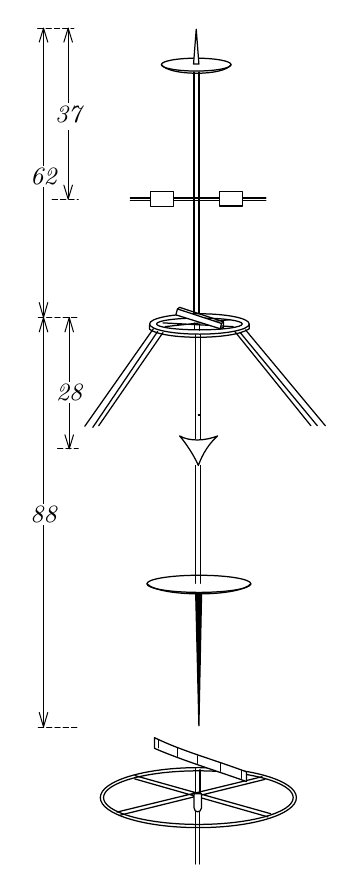
\begin{tikzpicture}[x=.0068cm,y=-.0068cm,line width=.45pt,line cap=round,line join=round]
\draw[line width=.28pt] (40,38)--(40,578) (40,578)--(40,1342)
 (86,38)--(86,357) (88,578)--(88,823);
\draw[line width=.28pt,dash pattern=on 2pt off 1pt]
 (29,38)--(97,38) (56,357)--(105,357) (30,578)--(104,578)
 (66,823)--(105,823) (30,1342)--(105,1342);
\draw[line width=.36pt] (32,64)--(40,38)--(48,64)
 (32,550)--(40,578)--(48,550) (32,605)--(40,578)--(48,605)
 (32,1315)--(40,1342)--(48,1315)
 (78,64)--(86,38)--(94,64) (78,331)--(86,357)--(94,331)
 (80,605)--(88,578)--(96,605) (80,797)--(88,823)--(96,797);
\node[fill=white,inner sep=1pt,font=\small\itshape] at (40,315) {62};
\node[fill=white,inner sep=1pt,font=\small\itshape] at (86,203) {37};
\node[fill=white,inner sep=1pt,font=\small\itshape] at (88,718) {28};
\node[fill=white,inner sep=1pt,font=\small\itshape] at (40,946) {88};
\draw (321,120)--(321,572) (330,120)--(330,574);
\draw (325,106) ellipse[x radius=65,y radius=12];
\draw (260,106)..controls(273,127)and(377,128)..(390,106);
\draw[fill=white] (320,105)--(325,40)--(330,105)--cycle;
\draw (202,355)--(455,355) (202,360)--(455,360);
\draw[fill=white] (239,343) rectangle (283,371);
\draw[fill=white] (368,343) rectangle (411,370);
\draw (245,599)--(117,781) (253,604)--(132,783) (263,606)--(143,780)
 (397,604)--(539,780) (407,606)--(551,780) (417,601)--(566,780);
\draw (324,610)--(324,804) (333,610)--(333,805)
 (324,854)--(324,1074) (333,854)--(333,1074);
\draw[fill=white] (331,590) ellipse[x radius=93,y radius=19];
\draw (238,592)--(238,600)..controls(265,620)and(394,620)..(424,599)--(424,591);
\draw (331,590) ellipse[x radius=80,y radius=11];
\draw (263,588)--(394,595) (267,595)--(388,582);
\draw[fill=white] (290,562)--(372,589)--(370,599)--(287,573)--cycle;
\draw (290,562)--(294,559)--(376,586)--(372,589) (370,599)--(376,596)--(376,586);
\draw (322,588)--(322,600) (331,592)--(331,602);
\draw (329,760)--(333,760);
\draw[fill=white] (294,799)..controls(307,814)and(321,836)..(329,854)
 ..controls(337,832)and(349,813)..(365,799)
 ..controls(342,808)and(314,810)..cycle;
\draw (330,1075) ellipse[x radius=97,y radius=16];
\draw (233,1075)..controls(258,1100)and(404,1100)..(427,1075);
\draw[fill=black] (324,1092)--(330,1340)--(335,1092)--cycle;
\draw (323,1420)--(323,1466) (332,1422)--(332,1467)
 (323,1498)--(323,1598) (331,1498)--(331,1598);
\draw (329,1474) ellipse[x radius=183,y radius=56];
\draw (329,1474) ellipse[x radius=177,y radius=50];
\draw (211,1433)--(464,1504) (210,1439)--(459,1510)
 (177,1501)--(448,1435) (182,1507)--(453,1440);
\draw[fill=white] (321,1467)--(335,1467)--(335,1493)
 ..controls(334,1503)and(321,1503)..(321,1493)--cycle;
\draw[fill=white] (247,1362)..controls(298,1387)and(355,1402)..(419,1426)
 --(419,1444)..controls(354,1421)and(298,1404)..(247,1382)--cycle;
\draw (254,1367)--(254,1381) (290,1382)--(290,1397)
 (328,1396)--(328,1410) (370,1410)--(370,1425) (410,1423)--(410,1438);
\end{tikzpicture}
\end{minipage}\par\noindent
Apparat ruht in einem hölzernen Gestell von $2{,}50$ m Höhe; eine eingravierte Inschrift
bezeichnet 1853, also kurz vor \textsc{Gauss}’ Tode, als das Konstruktionsjahr.

Ob \textsc{Gauss} noch mit diesem Instrument gearbeitet hat, ist nicht bekannt,
doch deuten manche Unvollkommenheiten darauf hin, dass es nicht geschehen ist.
Die Idee dieses Pendels ist aber weitergeführt worden; zunächst entwickelten
\textsc{Samter}\footnote{\textsc{Heinrich Samter}, \textit{Theorie des Gaussschen Pendels mit Rücksicht auf die Rotation der Erde.}
Diss. Leipzig 1886.} und \textsc{Lorentzen}\footnote{G. \textsc{Lorentzen}, \textit{Theorie des Gaussschen Pendels.} Astron. Nachr. 114, 1886, S. 241—284} seine Theorie, deren Hauptschwierigkeit in der Behandlung
der cardanischen Schneidenaufhängung besteht. Die Fehlerquellen sind
folgende: 1. die untere Schneide wird nicht genau horizontal liegen, 2. die
beiden Schneiden werden sich nicht genau rechtwinklig kreuzen und 3. nicht
in der gleichen Ebene liegen. Der erste Fehler bedingt eine zur Zeit pro\nobreakdash-
\clearpage\SourceLeaf{651}\ArithmeticHead{16}{L}{H. GEPPERT, ÜBER GAUSS’ ARBEITEN ZUR MECHANIK UND POTENTIALTHEORIE.}
\noindent portionale Störung der Azimutalbewegung, der zweite äussert sich in einer
Bevorzugung gewisser Azimute, und der dritte bedingt solche Störungen, dass
der \textsc{Foucault}sche Versuch mit dem \textsc{Gauss}schen Pendel nur dann gelingen
kann, wenn der Abstand der beiden Schneiden höchstens einige Mikron beträgt.
Somit gelingen diese Versuche nur bei Anwendung äusserster Vorsicht.
\textsc{Kamerlingh-Onnes}\footnote{H. \textsc{Kamerlingh-Onnes}, \textit{Nieuwe Bewijzen voor de Aswenteling der Aarde.} Diss. Groningen, 1879.} hat auf dieser Grundlage ein neues Pendel konstruiert,
indem er von dem \textsc{Gauss}schen Pendel die Idee der cardanischen Aufhängung,
der kurzen Pendellänge und der Spiegelablesung übernahm; eine geniale Abänderung
der Schneidenaufhängung gestattete ihm, den Abstand der Schneiden
zu Null zu machen; überdies schwingt sein Pendel im luftleeren Raum. Zwei
der Hauptträgheitsmomente ($A$ und $B$) waren nicht gleich, sondern um eine
Grösse 1. Ordnung verschieden, wodurch sich andere als die \textsc{Foucault}schen
Bahnen ergaben. Den Einfluss der Reibung und der endlichen Ausschläge
kann man dadurch beseitigen, dass man je zwei Versuche in zueinander senkrechten
Azimuten mittelt. Der \textsc{Kamerlingh-Onnes}sche Apparat ergibt sehr
präzise, mit der Theorie übereinstimmende Resultate.
\clearpage\endgroup
